% Source of the figure graph-classes.pdf: the class DC_2 with the graphs of diameter at most two and the graphs of
% cut-value at most two (cactus graphs), which overlap in C_4, and the two counterexamples (a) and (b) outside both.
% Compile with pdfLaTeX; the PDF is included in the manuscript at its natural size.
\documentclass[tikz,border=1pt]{standalone}
\usepackage[T1]{fontenc}
\pdfinfoomitdate=1 \pdftrailerid{} \pdfsuppressptexinfo=-1
\tikzset{
  vertex/.style={circle, fill=black, inner sep=0pt, minimum size=2.2mm},
  region/.style={line width=0.8pt, draw=black!75}}
\begin{document}
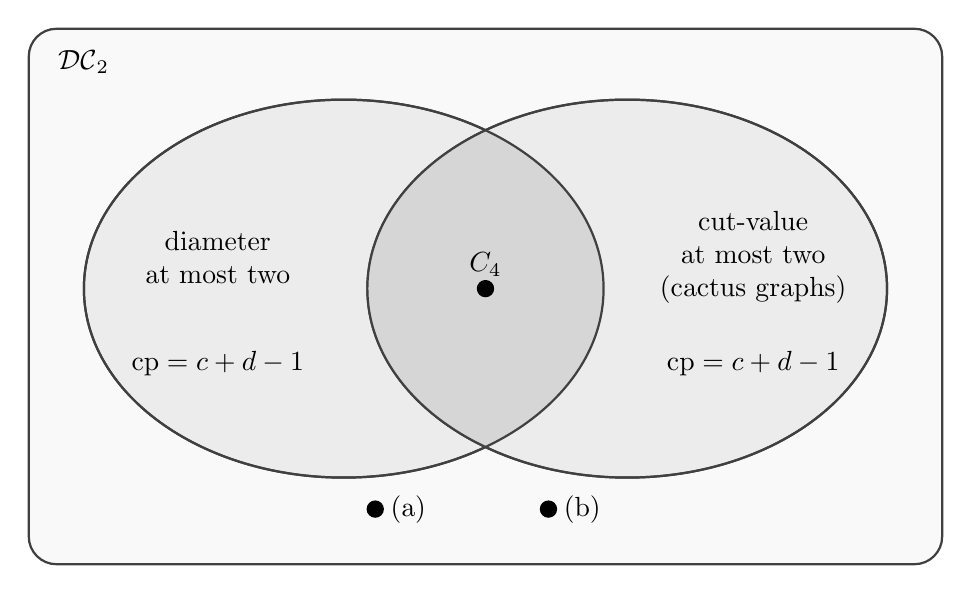
\begin{tikzpicture}[x=1cm, y=1cm]
  % the class DC_2
  \draw[region, rounded corners=10pt, fill=gray!5] (0,0) rectangle (11.6,6.8);
  \node[anchor=north west] at (0.25,6.65) {$\mathcal{DC}_2$};
  % the two inner classes; the overlap is shaded darker
  \draw[region, fill=gray!15] (4.0,3.5) ellipse[x radius=3.3, y radius=2.4];
  \draw[region, fill=gray!15] (7.6,3.5) ellipse[x radius=3.3, y radius=2.4];
  \begin{scope}
    \clip (4.0,3.5) ellipse[x radius=3.3, y radius=2.4];
    \fill[gray!32] (7.6,3.5) ellipse[x radius=3.3, y radius=2.4];
  \end{scope}
  \draw[region] (4.0,3.5) ellipse[x radius=3.3, y radius=2.4];
  \draw[region] (7.6,3.5) ellipse[x radius=3.3, y radius=2.4];
  % names and formula of the inner classes
  \node[align=center] at (2.4,3.9) {diameter\\at most two};
  \node at (2.4,2.55) {$\mathrm{cp}=c+d-1$};
  \node[align=center] at (9.2,3.9) {cut-value\\at most two\\(cactus graphs)};
  \node at (9.2,2.55) {$\mathrm{cp}=c+d-1$};
  % the cycle on four vertices lies in both
  \node[vertex] (c4) at (5.8,3.5) {};
  \node[above=1pt] at (c4) {$C_4$};
  % the counterexamples lie in neither
  \node[vertex] (pa) at (4.4,0.7) {};
  \node[right=2pt] at (pa) {(a)};
  \node[vertex] (pb) at (6.6,0.7) {};
  \node[right=2pt] at (pb) {(b)};
\end{tikzpicture}
\end{document}
